\documentclass{beamer}

\usetheme{Darmstadt}
\usepackage{amsfonts}
\usepackage{graphics,xcolor}
\usepackage{stmaryrd,amssymb,amsmath}
\usepackage[most]{tcolorbox}
\newtcolorbox{lol}[1]{colback=red!5!white,colframe=red!75!black,fonttitle=\bfseries,title=#1,breakable}
\usepackage{docmute}
\usepackage{hyperref}
\usepackage{graphicx}
%\usepackage{unicode-math}
\newcommand{\nat}{\mathbb{N}}
\newcommand{\ints}{\mathbb{Z}}
\newcommand{\intersection}{\ensuremath{\cap}}
\newcommand{\emptyword}{\ensuremath{\epsilon}}
\newcommand{\len}[1]{\ensuremath{|#1|}}
\newcommand{\union}{\ensuremath{\cup}}
\newcommand{\deltahat}{\ensuremath{\widehat{\delta}}}


\title{GPU Architcture}

\author{Balaji}
\date{}
\institute{IISc Bangalore}
\begin{document}
\maketitle
\section{Parallelism In GPUs}
\begin{frame}{Building blocks}
    \begin{itemize}
        \item Thread- program, line to be executed, data structures, values of variables
        \item Block- A collection of threads in the \textbf{grid}. Flexibility in the number of threads in a block. 
        \item Warp - 32 threads in a block, executed in parallel. \_\_syncthreads() to synchronize threads in a block. \_\_syncwarp() to synchronize warps.
        \item x,y,z dimensions of thread, block ids
        \item SM - streaming multiprocessors, having cuda cores.
        \item SPMD vs SIMD - Single Program Multiple Data vs Single Instruction Multiple Data
    \end{itemize}
    
\end{frame}
\begin{frame}{Kernel Functions}
    \begin{itemize}
        \item A function that is executed on the GPU
        \item Keywords: \_\_global\_\_, \_\_device\_\_, \_\_host\_\_, \_\_shared\_\_
        \item cudaMalloc / cudaFree ,cudaMemcpy to allocate/free memory on the GPU and transfer data between CPU and GPU respectively
        \item Called as kernelName<<<blockspergrid, threadsperblock>>>(args)
        \item Compiled by nvcc compiler to generate PTX code which is further compiled into an object file executed on GPU.
        \item Dynamically allocated arrays cant be multidimensional, have to be linearized.
    \end{itemize}
\end{frame}
\section{GPU Scheduling}

\begin{frame}{Transparent Scalability}
    \begin{itemize}
        \item Barrier to be synchronized so that all threads reach same execution point.
        \item Only for threads in a block, so multiple blocks can be parallelly executed.
        \item Threads waiting for each other to reach the same checkpoint- deadlock
        \item The ability to execute the same application code on different hardware with different
        amounts of execution resources is referred to as transparent scalability
    \end{itemize}
\end{frame}
\begin{frame}{Warps And SIMD}
    \begin{itemize}
        \item Single instruction executed by a all threads in a warp.
        \item Cores in SM arranged into processing blocks.
        \item Each warp is assigned to the same processing block. 
        \item Lesser area for control, more for arithmetic throughput.
    \end{itemize}
\end{frame}
\begin{frame}{Control Divergence}
    \begin{itemize}
        \item If threads in a warp take different paths, SIMD mechanism takes multiple passes.
        \item These multiple passes are executed sequentially or parallely in different gpu architectures.
        \item Each thread follows its own control flow and in a pass corresponding to an instruction it does not follow, the thread becomes inactive.
    \end{itemize}
\end{frame}
\begin{frame}{Reducing Latency In GPUs}
    \begin{itemize}
        \item Zero-overhead Scheduling in GPUs- Puts long latency operation warps to sleep and finds another warp to execute.
        \item Subscribes to a lot more threads than executable using available resources(cores,registers) on SM, to find a warp that can be executed while a warp is executing a long latency operation.
        \item GPUs can dedicate more chip area to floating-point execution and memory access channel resources than cache memory and branch prediction mechanisms.
        \item The ratio of the number of warps assigned to an SM to the maximum number it supports is referred to as occupancy.
    \end{itemize}
\end{frame}
\begin{frame}{Limitations to occupancy}
    \begin{itemize}
        \item Dynamic block partitioning(Variable number of threads) in GPUs to allocates exact amount of resources as per requirements
        \item Number of threads that can be supported by SM not being multiple of threads per block 
        \item Maximum number of blocks that can be assigned to SM is limited.
        \item Blocks executing code with lot of automatic variables having register requirements can reduce occupancy. Limit in registers per SM.
        \item Register spilling to local memory may increase execution time.
        \item Shared Memory usage by blocks similarly.
    \end{itemize}
\end{frame}
\section{Memory types}
\begin{frame}{Efficiency Barrier}
    \begin{center}
    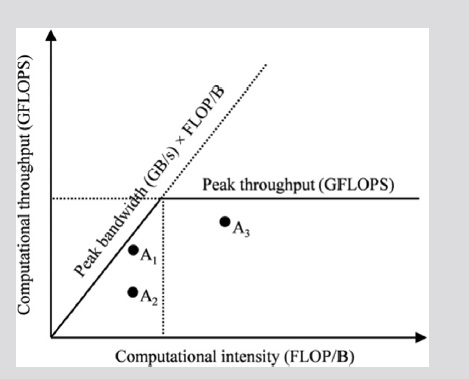
\includegraphics[scale = 0.4]{Barrier}
    \end{center}
    \begin{itemize}
    \item Compute to global memory access ratio is called computational intensity.
    \item Memory bandwidth limits throughput of memory-bound programs.
    \item Higher computational intense programs are compute-bound by the hardware resources, lower ones are memory-bound.
    \end{itemize}
\end{frame}
\begin{frame}{Memory types in GPU}
    \begin{itemize}
        \item Global memory - accessible by all threads, slow, large, read and write
        \item Local Memory - portion of the global memory reserved by a thread, eg: statically allocated arrays, spilled registers, and other elements of the
        thread’s call stack.
        \item Shared memory - accessible by threads in a block, fast, small
        \item Constant memory - read only, short-latency, high-bandwidth, read-only-access for the device, writable by host
        \item Register memory - fast, small, per thread
        \item Texture memory - Not discussed
        
    \end{itemize}
    
\end{frame}
\begin{frame}{Locations And Access}
    \begin{center}
    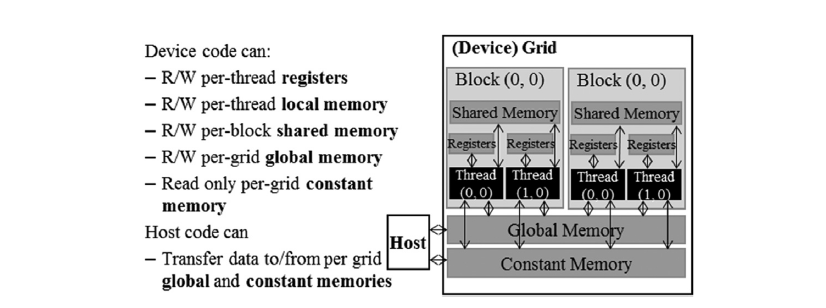
\includegraphics[scale = 0.4]{Location}
    \end{center}
    \begin{center}
    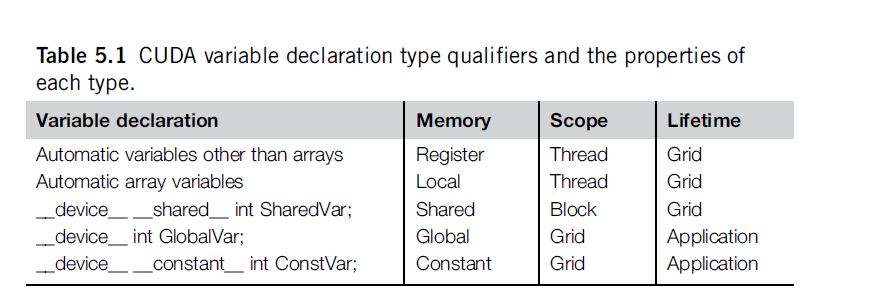
\includegraphics[scale = 0.4]{Occupancy}
    \end{center}

\end{frame}
\begin{frame}{Shared memory block optimisations}
    \begin{itemize}
        \item Usage of locality(on-chip constant caching), tiling algorithms to utilize shared memory reduce latency.
        \item Strip Mining - breaking a large problem into smaller ones that fit into shared memory.
        \item Can compute appropriate shared memory per block using cuda. Declaring an extern array will dynamically allocate an array of a given siize without mentioning the same. 
        \item Do boundary checking of tiling algorithms when matrices multiplied are rectangular and dimensions are not multiples of tile width.
    \end{itemize}
\end{frame}
\end{document}